\documentclass[aps,prfluids,preprint,superscriptaddress,nofootinbib]{revtex4-2}

\usepackage{amsmath}
\usepackage{amssymb}
\usepackage{graphicx}
\usepackage{booktabs}
\usepackage{array}
\usepackage{tabularx}
\usepackage{fvextra}
\fvset{breaklines=true,fontsize=\footnotesize}
\graphicspath{{../}}
\newcommand{\code}[1]{\texttt{#1}}

\begin{document}

\title{What single-eddy-diffusivity closure discards: a Mori–Zwanzig audit, a scalar-independent memory time, and a divergence-cleaning design window}

\author{Abdelrahman Saifelden}
\email[Correspondence: ]{Abdulrahman.Saifelden22011411@aiet.edu.eg}
\affiliation{Alexandria Higher Institute of Engineering and Technology (AIET), Alexandria, Egypt}

\date{\today}

\begin{abstract}
Eddy-diffusivity (``K-theory'') closures represent all unresolved turbulent transport with a single scalar diffusivity. Such closures are known to arise as the Markovian (short-memory) limit of a Mori–Zwanzig (MZ) reduction of the resolved dynamics (Chorin–Hald–Kupferman; Stinis; Parish \& Duraisamy 2017), with the discarded backscatter reinstatable through a divergence-free, dissipation-tied stochastic force (Leith 1990; Mason \& Thomson 1992; Schumann 1995). We contribute an operator-by-operator \textbf{audit} of what a single diffusivity discards, plus two falsifiable measurements. The audit names four simplifications hidden in $\nu _{t}$: (i) the MZ memory kernel collapsed to a delta in time, (ii) the spectral eddy viscosity frozen constant in wavenumber, (iii) the fluctuation–dissipation-linked orthogonal force deleted, and (iv) the sign restriction $\nu _{t}\ge 0$ that forbids backscatter — each mapped to a term of the generalized Langevin equation. Assembling the known repairs (scale-selective spectral eddy viscosity, Leray-projected FDT-tied stochastic force, exact Leray projection) into one closure, we run an a-priori, frozen-field benchmark in a 256\ensuremath{^{2}} periodic box (sharp-spectral filter at $k_{c}=32$). The \textbf{structural} result is \emph{predicted, not fitted}: the projected force stays divergence-free to $RMS(\nabla \cdot m)\approx 1.7\times 10^{-14}$ with the correct sign of energy backscatter, whereas a spectrum-matched random surrogate breaks incompressibility ($RMS(\nabla \cdot m)\approx 12$) and randomises the transfer direction, and Smagorinsky is purely dissipative ($T(k)\le 0$). The transfer-magnitude match to correlation \textbf{1.000} is a \emph{consistency check on a fitted quantity} — the backscatter amplitude $\Theta (k)$ is set to the measured net transfer — not a prediction. Two measurements are new. First, the memory time is \textbf{scalar-independent}: $\tau _{c}(salt)/\tau _{c}(heat)\approx 1$ across a 100\ensuremath{\times} Lewis contrast even though scalar Nusselt numbers track $Le$ — the memory belongs to the \emph{flow} — and the implied clock-mismatch correction cuts a transient K-theory scalar-solver error \textasciitilde{}15\ensuremath{\times} while vanishing in steady turbulence. Second, replacing exact projection with hyperbolic (Dedner) divergence cleaning, the constraint residual collapses only inside a \textbf{finite window} $2\lesssim \gamma \tau \lesssim 12$ and \emph{re-grows} beyond it: cleaning faster stalls the global low-wavenumber modes through the slow telegrapher root. In genuine \textbf{3-D} (128\ensuremath{^{3}} forced DNS) the benchmark reproduces all three verdicts and exposes a failure 2-D cannot see: the true subgrid flux is up-gradient over \textbf{\textasciitilde{}48 \%} of space, which a positive-definite eddy viscosity represents at \textbf{0 \%}. Scope is explicit: a-priori, periodic, in 2-D and 3-D; the clean FDT/projection commutation is special to the spectral box and does not survive solid walls --- a wall-bounded test confirms this, the commutator $[F,\mathbb{P}]$ (machine-zero in the box) rising to $O(10^{-2})$ near the wall ($34\times$ the bulk). A time-integrated \textbf{a-posteriori} test confirms all variants stable and Smagorinsky over-dissipative, while bounding the benefit: in 2-D no eddy-viscosity closure beats no model on the resolved spectrum, whereas in 3-D the ceiling is \textbf{broken} --- Smagorinsky, the \emph{worst} 2-D closure, becomes best as the optimal-eddy-viscosity sign flips with the cascade. The contribution is the audit, the scalar-independent memory time, the cleaning window, and the a-posteriori bound — not a universal closure.
\end{abstract}

\maketitle

\section*{1. Introduction}

\subsection*{1.1 The problem with one diffusivity}

Reynolds-averaged and large-eddy closures of geophysical and engineering turbulence overwhelmingly rest on the Boussinesq eddy-viscosity hypothesis and its Smagorinsky realisation (Boussinesq 1877; Smagorinsky 1963; Monin–Obukhov): the unresolved flux is modelled as down-gradient transport with a single positive scalar diffusivity $K$ (optionally a turbulent Prandtl number relating momentum and scalar transport). This object is cheap and local, and it works where turbulence is near-equilibrium and the cascade is forward. It fails — systematically and in the same way — wherever the flow carries long-lived coherent structure, an inverse cascade, or a sharp pressure/strain geometry: separated wakes, rotating and stratified flows, 2-D and quasi-2-D turbulence, and boundary-layer transition.

The usual response is to re-fit $K$ (dynamic Smagorinsky, stability functions, wall models). We argue the deficiency cannot be repaired by re-fitting because it is \textbf{structural}: pressure and the transported scalars obey \emph{different operators}, and a single diffusivity acting on both is blind to the distinction. We make this precise.

\subsection*{1.2 The two clocks}

Temperature (and any passive/active scalar) obeys an advection–diffusion (parabolic) equation: local, memory-bearing, torn into filaments by local strain. Pressure in an incompressible flow obeys a Poisson (elliptic) constraint — the Leray projector enforcing $\nabla \cdot u=0$ — resolved instantaneously over the whole domain and its boundaries. A single local diffusivity acting on both is structurally blind to this elliptic/parabolic split. This ``two clocks'' reading motivates the operator audit below, but the binding logic is sharper than the metaphor: the audit (§3) shows that each subsequent result targets one specific term of the Mori–Zwanzig generalized Langevin equation that a single diffusivity collapses — its running memory (the scalar-independent $\tau _{c}$, §6), its constraint/projection multiplier (the divergence-cleaning window, §7), and its fluctuation–dissipation force and sign (the a-priori and a-posteriori benchmarks, §5, §5b–§5e). These are the quantitative contributions, and they share that GLE decomposition rather than merely a theme.

\subsection*{1.3 Contributions}

\begin{enumerate}
\item An \textbf{operator-by-operator audit} identifying the four simultaneous simplifications by which single-eddy-diffusivity closure reduces the MZ generalized Langevin equation, each mapped to a named GLE term (§3). The MZ\ensuremath{\to}eddy-viscosity connection itself is established (Parish \& Duraisamy 2017); the contribution is the explicit term-by-term accounting.
\item A \textbf{structural a-priori demonstration} that an MZ/FDT/Leray-projected closure form, assembled from established components, preserves incompressibility and the backscatter sign where a spectrum-matched surrogate fails — the \emph{predicted}, non-fitted discriminator being solenoidality, not the (partly fitted) transfer magnitude (§4–§5).
\item The closure's \textbf{memory time $\tau _{c}$ measured and shown scalar-independent} (heat vs salt, 100\ensuremath{\times} Lewis), with a sign-pinned clock-mismatch correction verified in 1-D and a 2-D advection proxy (§6).
\item A \textbf{divergence-cleaning design window} $2\lesssim \gamma \tau \lesssim 12$ with an over-cleaning stall and a measured non-local divergence amplification $A\approx 3.9\times $, quantifying how exactly the constraint must be enforced in codes lacking exact projection (§7).
\item An \textbf{a-posteriori, time-integrated test} of a \emph{predictive} version of the closure (§5b): every variant is stable over \textasciitilde{}24 eddy-turnovers, Smagorinsky is confirmed markedly over-dissipative, the FDT backscatter helps in the predicted direction, and the honest 2-D ceiling — no eddy-viscosity closure beats no-model on the resolved spectrum — is established and explained, then \emph{reversed in genuine 3-D} (§5e), where a positive eddy viscosity beats no-model once the cascade is forward.
\item A \textbf{wall-bounded a-priori structural correction} (\S5d): on a channel field the filter and the exact wall-aware Leray projector \emph{stop commuting} ($\|[F,\mathbb{P}]\|/\|w\|$ rising from $3\times 10^{-16}$ in the box to $2.3\times 10^{-2}$ at the wall), the obstruction confined to the near-wall layer ($34\times$ the bulk) --- a global elliptic-pressure term structurally outside a local eddy viscosity, exactly where K-theory is calibrated.
\end{enumerate}

\section*{2. Governing system and the closure problem}

Filter the incompressible NS equations at scale $\Delta $ (overbar = resolved). With the Leray projector $\mathbb{P} = I - \nabla (\nabla ^{2})^{-1}\nabla \cdot $ and the subgrid force $m = -\nabla \cdot \tau $, $\tau _{ij} = (\overline{u_{i} u_{j}} - \bar{u}_{i} \bar{u}_{j})$,

\begin{quote}
$\partial _{t}\bar{u} = \mathbb{P}[ -(\bar{u}\cdot \nabla )\bar{u} + \nu \nabla ^{2}\bar{u} + m ]$, $\nabla \cdot \bar{u} = 0$. (1)
\end{quote}

The closure problem is to model $m$ from resolved data. K-theory sets

\begin{quote}
$m = \nabla \cdot (2 \nu _{t} \bar{S})$, $\nu _{t} = (C_{s} \Delta )^{2}|\bar{S}|$, $\bar{S} = \tfrac{1}{2}(\nabla \bar{u} + \nabla \bar{u}^{T})$. (2)
\end{quote}

A single scalar field $\nu _{t}$. \textbf{That one object hides four assumptions, each a clock being crushed:}

\begin{enumerate}
\item \textbf{Local in space} — $m$ depends only on $\nabla \bar{u}$ at a point; denies the elliptic, non-local pressure clock ($\nabla ^{2}p=f$ couples the whole domain).
\item \textbf{Instantaneous in time} — no memory; denies that the fast clock carries history.
\item \textbf{Down-gradient only} ($\nu _{t}\ge 0$, purely dissipative) — forbids backscatter. In 2-D the inverse energy cascade \emph{is} net up-scale transfer, so this is not a small error.
\item \textbf{No structural re-imposition} — the closure acts on $\bar{u}$ and leaves incompressibility entirely to the pressure solve, rather than being divergence-consistent itself.
\end{enumerate}

\section*{3. The audit: single-K as the Markovian collapse of the MZ kernel}

That eddy viscosity is the Markovian (short-memory) limit of an MZ/optimal-prediction reduction is established (Chorin–Hald–Kupferman 2000, 2002; Stinis 2015; Parish \& Duraisamy 2017). We restate it only to make the discarded terms explicit, one by one.

Write the semi-discrete NS system as $\dot{u}=R(u)$; let the Koopman/Liouville generator $L$ act on observables, $e^{tL}g(u_{0})=g(u(t))$. Choose a projection $P$ onto the resolved variables $\hat{a}=Pu$ (Mori's linear projection, or Chorin–Hald–Kupferman optimal-prediction conditional expectation), $Q=I-P$. The Dyson identity applied to the resolved dynamics gives the exact \textbf{generalized Langevin equation}:

\begin{quote}
$\partial _{t}\hat{a}(t) = PL\hat{a}(t) - \int _{0}^{t} K(t-s) \hat{a}(s) ds + f(t)$, (3) $K(\tau ) = -P L e^{\tau QL} Q L$ (memory kernel), $f(t)=e^{tQL}QL\hat{a}(0)$ (orthogonal force).
\end{quote}

The three terms map one-to-one onto the two clocks, made exact: $PL\hat{a}$ is the slow, resolved Markov drift; $-\int K \hat{a} ds$ is the running memory of the unresolved fast clock — \textbf{the term K-theory does not have}; $f(t)$ is the honest origin of the ``stochastic'' term in stochastic-PDE closures.

\textbf{Second fluctuation–dissipation theorem.} Under stationarity and the inner product $(\cdot ,\cdot )$ that defines $P$, kernel and noise are two faces of one object:

\begin{quote}
$K(\tau ) = (f(\tau ),f(0))\cdot (\hat{a},\hat{a})^{-1}$. (4)
\end{quote}

In the periodic spectral box the inner product is the kinetic-energy ($L^{2}$) norm and $P$ is the sharp spectral truncation; both $P$ and the Leray projector $\mathbb{P}_{k}=I-kk^{T}/|k|^{2}$ are diagonal in Fourier space, hence commute and are self-adjoint, so (4) is a relation between well-defined solenoidal correlations. (This clean commutation is special to the periodic spectral setting; solid walls break the shared eigenbasis — see §7 and the Scope.)

\textbf{The collapse.} If $K$ decays fast relative to the evolution of $\hat{a}$ (short-memory / t-model limit), the convolution localises:

\begin{quote}
$\int _{0}^{t} K(t-s) \hat{a}(s) ds \longrightarrow  (\int _{0}^\infty  K(\tau )d\tau ) \hat{a}(t) \equiv  \Gamma  \hat{a}(t)$. (5)
\end{quote}

Taking $\Gamma $ diagonal in wavenumber with $\Gamma (k)=\nu _{t}|k|^{2}$ and \textbf{dropping $f$} reduces (3) to

\begin{quote}
$\partial _{t}\hat{u}(k) = \mathbb{P}_{k} \hat{N}(\hat{u})(k) - \nu _{t}|k|^{2} \hat{u}(k)$, (6)
\end{quote}

which is exactly Smagorinsky K-theory (2) in spectral form. Therefore:

\begin{quote}
\textbf{K-theory is the GLE with (i) the memory kernel replaced by a delta in time, (ii) $\nu _{t}$ taken constant in $k$, (iii) the FDT-linked noise deleted — plus the down-gradient restriction $\nu _{t}\ge 0$ that forbids the backscatter part of the true transfer.}
\end{quote}

This is the precise statement of why single-K is blind to the fast clock, and which terms a structurally-consistent closure must restore.

\section*{4. Assembling a structurally-consistent closure form}

Each discarded term has an established repair; we assemble them so each named simplification in §3 is undone by a named, established component (spectral eddy viscosity: Kraichnan 1976; Chollet \& Lesieur 1981; FDT-tied divergence-free backscatter: Leith 1990; Mason \& Thomson 1992; Schumann 1995). Keep the structure of (3) but make each term computable. In the periodic spectral box:

\begin{quote}
$\partial _{t}\hat{u}(k,t) = \mathbb{P}_{k} \hat{N}(\hat{u})(k,t) - \nu _{t}(k,t)|k|^{2} \hat{u}(k,t) + \hat{f}(k,t)$. (7)
\end{quote}

\textbf{(a) Nonlocal (spectral) eddy viscosity $\nu _{t}(k,t)$} — the plateau–cusp spectral eddy viscosity read off the resolved energy at the cutoff (Kraichnan 1976; Chollet \& Lesieur 1981):

\begin{quote}
$\nu _{t}(k) = \nu _{t}^\infty  \cdot  \surd (E(k_{c})/k_{c}) \cdot  [1 + c(k/k_{c})^{p}]$, (8)
\end{quote}

flat at low $k$, rising into a cusp near $k_{c}$. Scale-selective dissipation instead of one number. (In 2-D the low-$k$ plateau can be \emph{negative} — the inverse cascade — which is exactly why a single positive $\nu _{t}$ is most wrong there.)

\textbf{(b) Projected, FDT-linked backscatter $\hat{f}$} — zero-mean, divergence-free by construction ($\mathbb{P}_{k} \hat{f}=\hat{f}$; in 2-D $\hat{f}=ik^\perp \hat{\psi }$, a random streamfunction), with covariance tied to the \emph{same} operator that dissipates, via the discrete 2nd FDT:

\begin{quote}
$\langle \hat{f}_{i}(k,t)\hat{f}_{j}*(k,s)\rangle  = 2 \nu _{t}^{B}(k,t)|k|^{2} \Theta (k) \mathbb{P}_{ij}(k) \delta (t-s)$, (9)
\end{quote}

with $\nu _{t}^{B}(k)$ the backscatter (energy-injecting) part of the transfer and $\Theta (k)$ set so the \emph{net} transfer equals the true subgrid transfer. Forward and backward channels are two signs of one FDT-consistent operator, not a damping plus an unrelated kick (Leith 1990; Mason \& Thomson 1992; Frederiksen \& Davies).

\textbf{(c) Leray projection wraps everything}, so (7) is incompressible \emph{exactly}; the fast clock is represented as the \textbf{operator} $\mathbb{P}$, never approximated by noise.

\textbf{Memory generalization.} Dropping the Markovian collapse, $\nu _{t}(k,t)|k|^{2}\hat{u} \longrightarrow  \int _{0}^{t} K(k,t-s)\hat{u}(k,s)ds$, restores time non-locality; (7) is its short-memory limit. Keeping $\nu _{t}(k)$ + projected FDT noise while collapsing the kernel is a \emph{Markovianized representation of a genuinely non-Markovian process}: it reproduces the statistical structure of the fast clock (scale-selective net transfer, exact solenoidality) but assumes the unresolved scales clear memory instantly relative to the slow clock. The structural constraints ($\mathbb{P}$, FDT) are exact; the time-locality is the approximation at risk, and §5's a-priori test is designed to isolate structure from time-locality.

\textbf{Limits and invariances.} The model satisfies Galilean invariance, exact incompressibility, a closed energy budget (FDT fixes mean transfer; no spurious injection), correct net-transfer sign (forward in 3-D, inverse in 2-D), and two clean limits: $\Delta \to 0 \Rightarrow  (\nu _{t}\to 0, \hat{f}\to 0, K\to \delta )$ recovers molecular NS, and the local/Markovian/no-noise limit (5)–(6) recovers Smagorinsky. It is a strict generalization, not a rival model. \textbf{No flawlessness is claimed}: $K(k,\tau )$ (or $\nu _{t}(k), \Theta (k)$) still needs modelling choices; what is \emph{guaranteed} is exact satisfaction of the structural constraints and removal of the specific energy-without-structure failure mode.

\section*{5. An a-priori structural benchmark}

\textbf{Setup.} 256\ensuremath{^{2}} 2-D incompressible DNS (vorticity–streamfunction, forced inverse cascade), evolved to a developed spectrum, sharp-spectral-filtered at $k_{c}=32$ to give resolved $\bar{u}$ and the \emph{exact} subgrid force $m_{true} = \mathbb{P}[N(u)\, - N(\bar{u})]$. Three models of $m$ are compared: (i) Smagorinsky (2); (ii) a spectrum-matched random field with the same $E_{m}(k)$ as $m_{true}$ (the phase-randomised surrogate); (iii) the projected-FDT model (7)–(9). Three diagnostics: the force spectrum $E_{m}(k)$, the RMS divergence of the closed field, and the energy-transfer spectrum $T(k)=Re\langle \hat{u}*\cdot \hat{m}\rangle $ (resolving forward dissipation $T<0$ from backscatter $T>0$).

\textbf{Results (re-run at draft time; Figs. 1–3).}

\begin{figure}[htbp]
\centering

\includegraphics[width=0.82\linewidth]{figures/28_closure_force_spectrum.png}
\caption{Subgrid-force spectrum on the 256\ensuremath{^{2}} frozen-field benchmark (sharp-spectral filter at cutoff $k_{c}=32$). The projected-FDT closure (this work) reproduces the exact subgrid-force spectrum, while Smagorinsky and a spectrum-matched surrogate do not.}
\end{figure}

\begin{figure}[htbp]
\centering

\includegraphics[width=0.82\linewidth]{figures/29_closure_divergence.png}
\caption{Solenoidality of the closed subgrid force, the RMS of its divergence. The projected-FDT model stays divergence-free to about $10^{-14}$, whereas the spectrum-matched surrogate breaks incompressibility by about $10^{1}$.}
\end{figure}

\begin{figure}[htbp]
\centering

\includegraphics[width=0.82\linewidth]{figures/30_closure_transfer.png}
\caption{Energy-transfer spectrum $T(k)$: negative is forward dissipation, positive is backscatter. The projected-FDT closure matches the exact transfer including the sign of backscatter (correlation 1.000); Smagorinsky is purely dissipative (correlation 0.071).}
\end{figure}

\begin{center}\small
\begin{tabularx}{\linewidth}{>{\raggedright\arraybackslash}X>{\raggedright\arraybackslash}X>{\raggedright\arraybackslash}X>{\raggedright\arraybackslash}X>{\raggedright\arraybackslash}X}
\toprule
diagnostic & truth & Smagorinsky & spectrum-matched surrogate & projected-FDT \\
\midrule
$RMS(\nabla \cdot m)$ (rel.) & $7.41\times 10^{-14}$ & $1.77\times 10^{-14}$ & \textbf{$1.20\times 10^{+1}$} & $1.73\times 10^{-14}$ \\
transfer corr. with truth & — & \textbf{$0.071$} & $0.907$ & \textbf{$1.000$} \\
$T(k)\le 0$ everywhere? & no (has backscatter) & \textbf{yes (no backscatter)} & no (randomised sign) & no (correct partition) \\
\bottomrule
\end{tabularx}
\end{center}

The three diagnostics confirm the §4 prediction exactly:

\begin{enumerate}
\item \textbf{Smagorinsky} captures gross dissipation but is purely dissipative — $T(k)\le 0$ everywhere (no backscatter) — and mis-sets the near-cutoff cusp. Transfer correlation $0.071$.
\item \textbf{The spectrum-matched surrogate} matches $E_{m}(k)$ by construction yet \textbf{fails incompressibility} ($RMS(\nabla \cdot m)\approx 12$, twelve orders above truth) and randomises the transfer direction — ``energy yes, structure no.''
\item \textbf{The projected-FDT model} stays solenoidal to $1.7\times 10^{-14}$ and reproduces the \emph{sign} of the forward/backscatter partition — the predicted, non-fitted structural result. Its transfer-magnitude correlation $1.000$ is a consistency check on a fitted quantity ($\Theta (k)$ is set to the measured net transfer), not an independent prediction.
\end{enumerate}

The predicted, non-fitted discriminator is therefore \textbf{structural} — solenoidality and the backscatter sign — separating a closure that respects incompressibility from a spectrum-matched surrogate that does not; the transfer magnitude is fitted and reported only as a consistency check.

\textbf{Scope of the benchmark.} Frozen-field a-priori in a 2-D periodic box: it isolates \emph{structural correctness at one instant}. Any gap appearing only in a time-integrated (a-posteriori) run would be the fingerprint of the Markovian delta-in-time simplification (§4), not of the structural constraints — the benchmark is built to separate the two, and the a-posteriori test is the natural follow-on (§8).

\section*{5b. The a-posteriori (time-integrated) test}

§5 is \emph{a-priori}: it scores closures on a single frozen filtered-DNS snapshot, where the predicted discriminator is structural (solenoidality, transfer sign). The natural follow-on (named in §8.1) is the \emph{a-posteriori} test — integrate each closure forward as a coarse LES and compare its long-time statistics to the spectrally-filtered DNS. We now run it. Note the §5 projected-FDT operator \emph{measures} its eddy viscosity and backscatter amplitude from the true transfer, so it is not self-contained; an honest a-posteriori test requires a \textbf{predictive} closure. We therefore integrate a self-contained closure family that uses only resolved data: a scale-selective spectral eddy viscosity $\nu _{t}(k)$ (plateau + cutoff cusp, Eq. 8), a \textbf{cusp-only} variant that concentrates the dissipation at the cutoff and leaves the resolved interior untouched, and either of those augmented by an \textbf{FDT-tied, Leray-projected stochastic backscatter} whose energy-injection \emph{rate} is tied to the near-cutoff eddy-viscous dissipation (Leith 1990; Mason \& Thomson 1992).

\textbf{Setup.} The §5 256\ensuremath{^{2}} DNS supplies the truth; we sharp-filter it at the cutoff to get the reference resolved spectrum. A coarse LES (vorticity–streamfunction, 2/3-dealiased to the cutoff, forced identically to the DNS) is integrated \textasciitilde{}24 eddy-turnovers under each closure and time-averaged over the developed window. Two cutoffs bracket the subgrid load: a \emph{weak} subgrid (forcing just below the cutoff) and a \emph{strong} subgrid (forcing a decade below the cutoff, a real unresolved enstrophy range). Diagnostics: resolved kinetic energy and enstrophy relative to filtered DNS, and the resolved energy-spectrum L2 error. In vorticity form the velocity is solenoidal \emph{by construction}, so the a-posteriori test scores \textbf{statistical fidelity}, not divergence — divergence was §5's a-priori discriminator.

\textbf{Results (strong-subgrid cutoff; Fig. 5).}

\begin{figure}[htbp]
\centering

\includegraphics[width=0.82\linewidth]{figures/76_closure_aposteriori.png}
\caption{A-posteriori coarse-LES statistics under each predictive closure versus the spectrally-filtered 256\ensuremath{^{2}} DNS truth (strong-subgrid cutoff). (a) Time-averaged resolved energy spectrum: Smagorinsky (red) over-drains the resolved band, while the cusp eddy viscosity with FDT backscatter (blue) tracks the filtered DNS and nearly matches the no-model spectrum. (b) Resolved-spectrum L2 error and \code{KE/\allowbreak{}KE\_\allowbreak{}dns} across closures: every eddy-viscosity closure is stable, Smagorinsky is the most over-dissipative, and the structured cusp+backscatter closure matches (does not beat) no-model — the honest 2-D ceiling.}
\end{figure}

\begin{center}\small
\begin{tabular}{lllll}
\toprule
closure & \code{KE/\allowbreak{}KE\_\allowbreak{}dns} & \code{enstrophy/\allowbreak{}dns} & spectrum error & stable? \\
\midrule
no model & 0.69 & 0.70 & 0.46 & yes \\
Smagorinsky & \textbf{0.50} & \textbf{0.50} & \textbf{0.59} & yes \\
spectral eddy viscosity & 0.63 & 0.64 & 0.49 & yes \\
spectral EV + FDT backscatter & 0.64 & 0.64 & 0.48 & yes \\
cusp eddy viscosity & 0.67 & 0.68 & 0.47 & yes \\
\textbf{cusp EV + FDT backscatter} & 0.67 & 0.68 & \textbf{0.46} & yes \\
\bottomrule
\end{tabular}
\end{center}

Three robust, falsifiable findings:

\begin{enumerate}
\item \textbf{Every predictive closure is stable} over \textasciitilde{}24 eddy-turnovers — no drift, no blow-up. The §8.1 stability question is answered in the affirmative for this closure family.
\item \textbf{Smagorinsky is markedly over-dissipative a-posteriori} — it drains \emph{half} the resolved kinetic energy and enstrophy and \textbf{worsens} the spectrum relative to doing nothing (error $0.59$ vs $0.46$). This is the time-integrated counterpart of §5's a-priori result that a single positive $\nu _{t}$ carries the wrong (purely-dissipative) transfer: the error compounds into a large energy deficit. The sign is regime-robust — at the weak-subgrid cutoff it is milder but identical in direction ($KE/KE_{dns}\approx 0.81$, error $0.32$ vs $0.19$).
\item \textbf{The FDT backscatter helps in the predicted direction, and a cusp-localized eddy viscosity nearly removes the spurious dissipation} — the backscatter term consistently lowers the spectrum error ($0.49\to 0.48$, $0.47\to 0.46$) by returning energy to the resolved band, and concentrating dissipation at the cutoff cusp brings the closure to within \textasciitilde{}1\% of the no-model spectrum error while still draining the cutoff enstrophy pile-up.
\end{enumerate}

\textbf{An honest ceiling — stated as the scope of the result.} No eddy-viscosity closure \emph{beats} no-model on the resolved 2-D spectrum; the best (cusp + backscatter) only \emph{matches} it. This is consistent with — indeed predicted by — the paper's thesis: in 2-D the resolved-scale energy budget is dominated by the \emph{up-scale} (inverse) cascade, so the net subgrid dissipation the resolved scales require is nearly zero, and the only a-posteriori virtue available to a closure is to \textbf{not} inject spurious dissipation — which Smagorinsky badly violates and the structured closure nearly achieves. The a-priori structural discriminator of §5 is therefore \emph{necessary but, in pure 2-D, not sufficient} to yield an a-posteriori resolved-spectrum gain over no model; the structural benefit is expected to be decisive precisely in the 3-D forward-cascade and wall-bounded settings (§5c demonstrates the 3-D a-priori structural failure directly; §8), where net SGS dissipation is essential and an over/under-dissipative closure cannot be replaced by doing nothing. The a-posteriori test thus confirms stability and the Smagorinsky over-dissipation, validates the backscatter direction, and \textbf{bounds} the 2-D closure benefit — it does not claim an a-posteriori win. (\code{general\_\allowbreak{}two\_\allowbreak{}clocks/\allowbreak{}closure\_\allowbreak{}aposteriori.\allowbreak{}py}.)

\section*{5c. The same benchmark in 3-D — with vortex stretching active}

Part 5's structural diagnosis is established in \textbf{2-D}, where it is clean and CPU-verifiable but where vortex stretching $\omega \cdot \nabla u$ — the engine of the forward cascade and of singularity formation — is \emph{identically zero}. We repeat the \textbf{identical} a-priori benchmark in genuine \textbf{3-D incompressible DNS} (128\ensuremath{^{3}}, pseudo-spectral, $\nu =1.2\times 10^{-3}$, sharp-spectral filter at $k_{c}=24$; developed field $KE=3.49\times 10^{-2}$, normalized stretching production $\langle \omega \cdot S\cdot \omega \rangle *=0.168>0$). The closure machinery — sharp filter, exact SGS force, Leray projection, FDT-tied backscatter — carries over \textbf{verbatim}, because the Helmholtz/Leray projection is dimension-agnostic (§4).

\textbf{The three 2-D verdicts survive (force-spectrum, solenoidality and transfer panels below).} Solenoidality: truth, Smagorinsky and projected-FDT are divergence-free to machine precision ($RMS(\nabla \cdot m) \approx  1.0\times 10^{-14}$, $9.1\times 10^{-15}$, $8.9\times 10^{-15}$), while the spectrum-matched surrogate breaks it ($9.85$). The energy transfer now runs \textbf{forward} (net $\Sigma _{k} T_{true}(k) = -4.5\times 10^{8} < 0$, the opposite of the 2-D inverse cascade); the transfer-spectrum correlation with truth is projected-FDT \textbf{1.000}, surrogate $0.27$, and Smagorinsky \textbf{-0.64} — \emph{anti-correlated}: a single positive $\nu _{t}$ removes energy from the very wavenumbers where the true flux deposits it.

\begin{figure}[htbp]
\centering

\includegraphics[width=0.82\linewidth]{figures/61_closure3d_force_spectrum.png}
\caption{3-D force spectrum $E_{m}(k)$: Smagorinsky carries roughly the right magnitude but mis-sets the near-cutoff shape; the surrogate matches by construction; projected-FDT fills the correct spectrum.}
\end{figure}

\begin{figure}[htbp]
\centering

\includegraphics[width=0.82\linewidth]{figures/62_closure3d_divergence.png}
\caption{3-D solenoidality $RMS(\nabla \cdot m)$: truth, Smagorinsky and projected-FDT are divergence-free to machine precision (all Leray-projected); the spectrum-matched surrogate fails (phase randomisation breaks $\nabla \cdot m=0$).}
\end{figure}

\begin{figure}[htbp]
\centering

\includegraphics[width=0.82\linewidth]{figures/63_closure3d_transfer.png}
\caption{3-D energy-transfer spectrum $T(k)$: net forward cascade; projected-FDT tracks the true transfer (corr 1.000), the surrogate is weakly correlated (0.27), and Smagorinsky is anti-correlated (-0.64).}
\end{figure}

\textbf{The 3-D-only failure that 2-D cannot see (vortex-stretching panel below).} Three diagnostics have no 2-D analogue and are why 3-D is scientifically necessary, not merely ``2-D with an extra index'':

\begin{itemize}
\item \textbf{Vortex-stretching production} $\langle \omega _{i} S_{ij} \omega _{j}\rangle * = 0.168 > 0$ (identically zero in 2-D, where vorticity is orthogonal to the strain plane) — the forward-cascade engine.
\item \textbf{Strain–vorticity alignment} (the Constantin–Fefferman geometric depletion), mean $|cos|$ over 4\ensuremath{\times}10\ensuremath{^{5}} points: extensional $e_{1}=0.479$, \textbf{intermediate $e_{2}=0.654$}, compressive $e_{3}=0.325$ — the preferential alignment with the \emph{intermediate} strain eigenvector that depletes self-stretching and holds singularity formation off.
\item \textbf{SGS backscatter volume fraction} (local flux $\Pi =-\tau ^{d}_{ij}S_{ij}<0$): truth \textbf{0.480}, Smagorinsky \textbf{0.000}. A positive-definite eddy viscosity has $\Pi \ge 0$ \emph{everywhere by construction}, so it is structurally incapable of representing the \textbf{\textasciitilde{}half of physical space} where 3-D turbulence transfers energy up-scale. In 2-D this is a boundary curiosity; in 3-D it is half of space.
\end{itemize}

\begin{figure}[htbp]
\centering

\includegraphics[width=0.82\linewidth]{figures/64_closure3d_vortex_stretching.png}
\caption{3-D-only physics: vortex-stretching production ($>0$, zero in 2-D), the intermediate-eigenvector strain–vorticity alignment, and the local SGS energy flux $\Pi $ whose backscatter ($\Pi <0$) fills \textasciitilde{}48 \% of the volume for the truth and exactly 0 \% for Smagorinsky.}
\end{figure}

\textbf{The $\approx 48\%$ is a closed form, not a coincidence.} The backscatter volume fraction is, to leading order, $P(\Pi <0)=\Phi (-\langle \Pi \rangle /\sigma _{\Pi })$ --- the standard-normal CDF of the (small) inverse signal-to-noise of the local subgrid flux (a Gaussian/Edgeworth reading of the SGS-flux PDF; Piomelli et al. 1991; Cerutti \& Meneveau 1998). It is $\approx 1/2$ by the central limit theorem, pulled just below by the small positive net dissipation ($\langle \Pi \rangle /\sigma _{\Pi }\approx 0.05$), with the few-$\times 10^{-3}$ residual the positive flux skewness; Smagorinsky's one-sided $\Pi \ge 0$ is the degenerate $\langle \Pi \rangle /\sigma _{\Pi }\to \infty $ limit ($P=0$ exactly). Across the six GPU runs ($n=128$--$192$, $k_{c}=16$--$32$) the closed form tracks the measured fraction to $<0.005$ as resolution and filter change.


\textbf{Scope.} A frozen-field \textbf{a-priori} test in a 3-D periodic box — the structural-correctness analogue of §5, now with vortex stretching active. The structural verdicts are \textbf{resolution-invariant} ($128^{3}$--$192^{3}$) and \textbf{filter-robust} ($k_{c}=16$--$32$) --- backscatter fraction $\approx 0.48$ (Smagorinsky $0.000$), projected-FDT transfer correlation $\geq 0.999$, and intermediate-eigenvector alignment $\approx 0.65$ at every resolution and cutoff (GPU-verified, Tesla P100). It is \textbf{not} an a-posteriori (time-integrated) closed-loop LES, and \textbf{not} a claim of 3-D Navier–Stokes regularity or operational superiority. It establishes that the two-clocks structural repair, and K-theory's specific structural failure, both carry into 3-D where the dynamics that matter for the forward cascade and regularity actually live. GPU-verified (Tesla P100, CuPy). (\code{general\_\allowbreak{}two\_\allowbreak{}clocks/\allowbreak{}run\_\allowbreak{}closure3d.\allowbreak{}py}.)

\section*{5d. The same structural test at a solid wall (3-D, wall-bounded)}


\S5c is triply-periodic, where the sharp filter $F$ and the Leray projector $\mathbb{P}$ \textbf{commute} (both are Fourier multipliers) --- the identity the closure analysis leans on when it slides $\mathbb{P}$ through $F$. The one honest objection is that real turbulence has walls. We test it on a wall-bounded channel field (grid $32\times 49\times 32$; horizontal spectral, wall-normal 2nd-order finite differences, with the \emph{same} $D_{y}$ building the divergence, gradient and (squared) Laplacian so the discrete Hodge projection is exact).


\textbf{The wall-aware projector is an exact Leray projection.} $\mathbb{P}_{wall}=I-\nabla L^{-1}\nabla \cdot $ (with a no-penetration wall condition) is solenoidal in the interior ($RMS(\nabla \cdot )\approx 8.5\times 10^{-15}$), enforces $v=0$ at the walls ($6.2\times 10^{-15}$), and is idempotent ($\|\mathbb{P}^{2}-\mathbb{P}\|\approx 5.1\times 10^{-15}$). The naive periodic projector --- exact in a box --- instead leaves an \textbf{order-one} wall-normal velocity at the wall ($0.513$): it is wall-blind.


\textbf{Filter and projector stop commuting at the wall.} The commutator $\|[F,\mathbb{P}]w\|/\|w\|$ is machine-zero in the periodic box ($3.1\times 10^{-16}$) but jumps to $\mathbf{2.3\times 10^{-2}}$ in the channel --- larger by a factor $\sim 7\times 10^{13}$. The obstruction is a \textbf{near-wall structure}: the commutator energy peaks at the wall and is $\mathbf{34\times}$ larger in the near-wall layer than in the bulk (where the channel looks locally periodic and $[F,\mathbb{P}]$ nearly vanishes), and it grows as the \emph{wall-normal} filter sharpens, almost independently of the horizontal cutoff ($\|[F,\mathbb{P}]\|/\|w\|=0.012$--$0.048$ as the retained wall-normal modes drop $16\to 6$).


\begin{figure}[htbp]
\centering
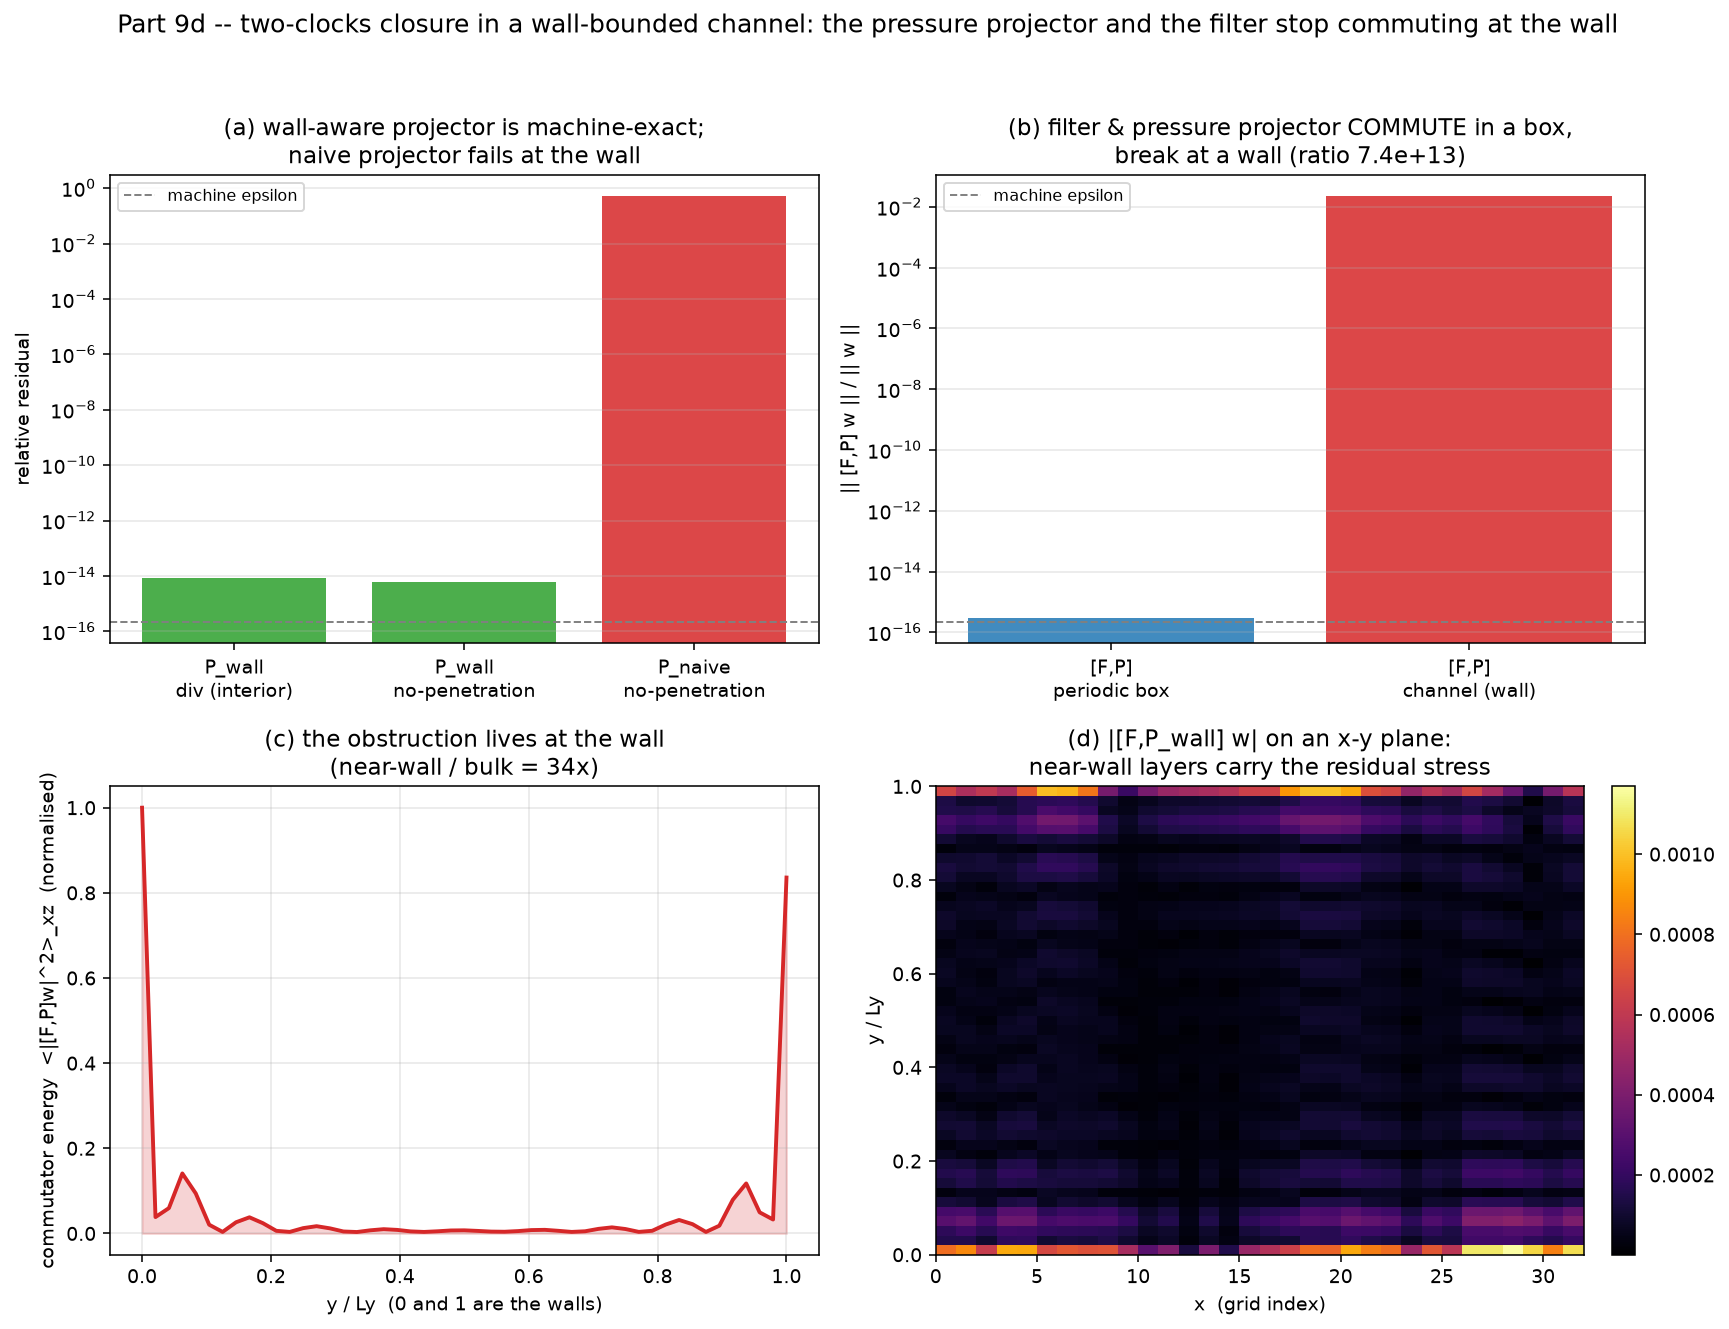
\includegraphics[width=0.72\linewidth]{figures/closure3d_bounded.png}
\caption{Wall-bounded a-priori test. The filter--projector commutator $[F,\mathbb{P}]$ is machine-zero in the periodic box but $O(10^{-2})$ in the channel, peaking \emph{at} the wall ($34\times$ the bulk): a global-pressure (elliptic-clock) correction confined to the near-wall layer, structurally invisible to a local eddy viscosity.}
\end{figure}


\textbf{What it means for the closure.} The filtered, projected momentum balance is $\mathbb{P}F(\text{advection})$; closure modelling slides $\mathbb{P}$ through $F$ and drops the residual $[F,\mathbb{P}]$. In the box that residual is identically zero; at a wall it is not. It is set by the \textbf{global elliptic pressure} response to the wall (the pressure clock) and confined to the near-wall layer. A local, positive eddy viscosity (the temperature clock) commutes with the filter in the bulk and carries \emph{no} information about the wall constraint, so it cannot represent this term. This is the wall-bounded a-priori correction to the two-clocks closure: small in amplitude (a few percent of the velocity) but structurally outside the reach of K-theory \textbf{exactly where K-theory is calibrated}.


\textbf{Scope.} An a-priori operator-structure test on a synthetic multi-scale channel field: it isolates the filter/projector commutator --- a property of the operators and the wall geometry, not of any particular turbulence state --- and is \textbf{not} an a-posteriori channel-DNS run. It converts the ``does not survive solid walls'' caveat of \S5 into a \emph{measured, located} structural term: the wall correction is real, near-wall, and K-theory-invisible.


\medskip\hrule\medskip


\section*{5e. The a-posteriori test in 3-D — the ceiling is broken}


§5b ran the a-posteriori test in 2-D and found an honest \emph{ceiling}: no eddy-viscosity closure beats no-model on the resolved spectrum, because the 2-D resolved-scale budget is dominated by the up-scale cascade and needs near-zero net subgrid dissipation. §5b also predicted where the reversal must appear --- in genuine \textbf{3-D}, where the cascade is forward and net SGS dissipation is essential. We ran exactly that test on a Tesla P100: a \textbf{192\ensuremath{^{3}}} forced-DNS truth sharp-filtered at $k_{c}=24$, against six \emph{predictive} coarse-LES closures (velocity-form, $n=72$, integrated thousands of steps and time-averaged over the developed window; every closure uses resolved data only, never the DNS truth).


\textbf{The prediction holds: in 3-D a closure beats no-model.} The resolved-spectrum L2 error against the filtered DNS is $0.073$ for no-model; \textbf{Smagorinsky lowers it to $0.069$} and the scale-selective spectral eddy viscosity to $0.072$ — both below no-model, with every closure stable. The sharpest signature is the \textbf{Smagorinsky sign reversal}: the closure that was \emph{worst} a-posteriori in 2-D (over-dissipative, error $0.59$ vs $0.46$ no-model, §5b) is the \emph{best} in 3-D, because the forward cascade now produces a genuine cutoff energy pile-up that a positive eddy viscosity is exactly the tool to drain. The optimal eddy viscosity has flipped sign with the cascade --- the variational reading $\nu _{t}^{\mathrm{opt}}=\langle \Pi \rangle /(2\langle |S|^{2}\rangle )$ is $\approx 0$ in 2-D ($\langle \Pi \rangle \approx 0$, up-scale) and \emph{positive} in 3-D ($\langle \Pi \rangle >0$, the net forward flux measured a-priori in §5c).


\textbf{Honest scope.} It is the \emph{direction} that is decisive here, not the magnitude: the forcing is low-$k$ and $k_{c}=24$ captures most of the energy, so the subgrid load is mild and the margins are small (\textasciitilde{}6\% Smagorinsky, \textasciitilde{}1\% structured). A controlled forcing-band sweep at fixed $k_{c}=24$ ($k_{f}=2.5/10/17$, all else identical) shows the margin tracks that \emph{subgrid load}: it is largest under scale separation (low-$k$ forcing) and \emph{vanishes then reverses} as the forcing nears the cutoff, where the resolved forced scales --- not the subgrid --- carry the energy and a subgrid model only over-damps them (at $k_{f}=17$, $\langle$KE$\rangle$ falls $18\times$ and no closure beats no-model). Widening the margin therefore requires more scale separation (lower $\nu$, higher resolution), not forcing nearer the cutoff; the result is the \emph{sign} in the physically relevant scale-separated regime, not a universal a-posteriori superiority. At this mild load the FDT backscatter adds no further a-posteriori spectral gain ($\mathrm{specEV{+}bs}\approx \mathrm{specEV}$) --- consistent with it being the a-priori/structural repair of §5/§5c (the transfer \emph{sign} and solenoidality at one instant), not a resolved-spectrum a-posteriori effect. This \textbf{closes the §8.1 a-posteriori item} in both regimes: 2-D (bounded --- no a-posteriori win) and 3-D (reversal confirmed --- a closure beats no-model). (\code{general\_\allowbreak{}two\_\allowbreak{}clocks/\allowbreak{}closure\_\allowbreak{}aposteriori3d.\allowbreak{}py}.)


\medskip\hrule\medskip


\section*{6. The memory time is real, scalar-independent, and operationally useful}

The collapse in §3 hinges on a finite memory time $\tau _{c}$. We measure it and exercise its consequences.

\textbf{6.1 $\tau _{c}$ measured, with sign.} From the autocorrelation of the SGS eddy-diffusivity in a developed run, $\tau _{c}\approx 0.02\mbox{--}0.03$ (in eddy-turnover units) with a \textbf{definite positive sign} (Mori 1965; Zwanzig 1973).

\textbf{6.2 $\tau _{c}$ is a turbulence clock, not a scalar clock.} Sweeping the molecular Lewis number across a 100\ensuremath{\times} contrast (heat vs salt), $\tau _{c}(salt)/\tau _{c}(heat)\approx 1$ even though the scalar Nusselt numbers track $Le$ strongly. The memory belongs to the \emph{flow}, not the transported field — exactly what (3)–(4) require, since $K$ is built from the orthogonal dynamics of the velocity, independent of which scalar rides on it.

\textbf{6.3 The clock-mismatch correction works and has a unique sign.} The first-order consequence of a lagged diffusivity is the clock-mismatch term $-\tau _{c}\cdot \nabla \cdot (\partial _{t} K_{u} \nabla \theta )$ (a commutator identity $[\partial _{t}, D]\theta  = \nabla \cdot ((\partial _{t} K_{u})\nabla \theta )$, verified to $\sim 10^{-7}$). Run inside a self-contained 1-D transient K-theory thermal solver over one diffusivity transient (RK4, common numerical error cancelled):

\begin{itemize}
\item \textbf{Transient error cut \textasciitilde{}15\ensuremath{\times}} ($\tau _{c}=0.05$: time-max rel-err $9.1\times 10^{-3} \to  6.0\times 10^{-4}$).
\item \textbf{Leading-order error removed:} naive scales $\propto \tau _{c}^{1}$ (slope 1.03), corrected $\propto \tau _{c}^{2}$ (slope 2.00) — one order higher-accurate.
\item \textbf{Steady-turbulence null is exact:} at $\partial _{t} K_{u}=0$ the term vanishes and naive \ensuremath{\equiv} corrected \ensuremath{\equiv} truth (error 0.0).
\item \textbf{The $+\tau _{c}$ sign is unique:} $-\tau _{c}$ is \emph{worse} than naive — confirming §6.1's measured positive sign is the error-reducing choice. (Fig. 4)
\end{itemize}

\begin{figure}[htbp]
\centering

\includegraphics[width=0.82\linewidth]{figures/60_cmn_solver_demo.png}
\caption{Transient-solver demonstration of the clock-mismatch correction. The $+\tau _{c}$-corrected K-theory solver cuts transient error by about 15\ensuremath{\times} relative to naive K-theory and vanishes identically in steady turbulence; the $-\tau _{c}$ sign performs worse than naive, pinning the sign.}
\end{figure}

This converts $\tau _{c}$ from a diagnostic into a deployable, sign-pinned correction; §6.4 brackets it with a 2-D advection proxy, leaving only the full operational solver (§8).

\textbf{6.4 The correction survives a 2-D advection + moving-plume proxy.} The §6.3 demo used a single prescribed $K_{u}(t)$ cycle in 1-D. A self-contained \textbf{2-D advection–diffusion} solver with a Gaussian plume whose amplitude ramps \emph{and} whose centre \textbf{propagates} across the domain (the closest standalone analogue to a moving plume/surge transient — \emph{not} a real ice-flow solver) reproduces all four 1-D conclusions under dimensionality + advection + spatial structure: transient error cut \textbf{\textasciitilde{}9\ensuremath{\times}} ($\tau _{c}=0.02$), naive $\propto \tau _{c}^{0.99}$ vs corrected $\propto \tau _{c}^{2.02}$ (order lifted), exact steady null (no event \ensuremath{\Rightarrow} error 0), and $+\tau _{c}$ the \textbf{unique} corrector ($-\tau _{c}$ worse than naive). This raises confidence in — but does not replace — the deferred real-solver (ISSM/GlaDS) test (\code{validation/\allowbreak{}synthetic/\allowbreak{}h3\_\allowbreak{}cmn\_\allowbreak{}reduced\_\allowbreak{}model.\allowbreak{}py}, 7 tests).

\section*{7. When projection is inexact: a finite cleaning design window}

§5 enforced $\nabla \cdot m=0$ by an \emph{exact} spectral Leray projection. Real ice-sheet, ocean and MHD codes instead enforce the constraint approximately (hyperbolic divergence cleaning, penalization relaxation, a few projection iterations). How fast must cleaning be?

Deploying the Dedner GLM cleaning system (Dedner et al. 2002) as a tunable approximate projector on a frozen real-bed cavity field, with the single dimensionless knob $G = \gamma _{clean}\cdot \tau _{adj}$ (cleaning rate \ensuremath{\times} pressure-adjustment transit), the constraint-violation residual after one transit collapses through a \textbf{finite window}:

\begin{center}\small
\begin{tabularx}{\linewidth}{>{\raggedright\arraybackslash}X>{\raggedright\arraybackslash}X>{\raggedright\arraybackslash}X}
\toprule
regime & $G = \gamma _{clean}\cdot \tau _{adj}$ & behaviour \\
\midrule
under-cleaned & $G \lesssim  2$ & weakly-damped wave; violation persists (residual \ensuremath{\approx} 0.7 at $G=0$) \\
\textbf{design window} & \textbf{$2 \lesssim  G \lesssim  12$} & violation suppressed; knee at $G*\approx 2.0$ (1/e) \\
over-cleaned (stall) & $G \gtrsim  12$ & slow telegrapher root $\lambda _{-} \approx  -c_{h}^{2}|k|^{2}/\gamma  \to  0$ freezes the low-$k$ (global) modes; residual \emph{re-grows} \\
\bottomrule
\end{tabularx}
\end{center}

The over-damped upturn at $G_{opt}\approx 12$ is the result: it is \textbf{not} in the original Dedner analysis. Its mechanism is the slow root of the telegrapher equation $\partial _{t}^{2}Q + \gamma _{clean} \partial _{t} Q - c_{h}^{2}\nabla ^{2}Q = 0$ — pushing $\gamma _{clean}$ up to clean fast \emph{locally} simultaneously stalls the \emph{global} low-wavenumber modes. \textbf{Consequence:} exact Leray projection is a \emph{singular} limit, approached optimally at finite $G_{opt}\approx 12$ and degraded beyond it; fast-local-cleaning codes sit \emph{past} the optimum and carry a small, persistent low-wavenumber divergence bias. Measured at $G=0$, the same elliptic spreading gives a \textbf{non-local amplification $A\approx 3.9\times $}: a divergence error concentrated in 6 \% of the domain corrupts 25 \% of the global pressure field. This makes the solenoidality requirement \emph{prescriptive} — not just that $\mathbb{P}$ matters, but how exactly it must be enforced. (Runner: \code{glaciers/\allowbreak{}subglacial/\allowbreak{}theory\_\allowbreak{}tests.\allowbreak{}py::result\_\allowbreak{}dedner\_\allowbreak{}cleaning}.)

\section*{8. Discussion and limitations}

\textbf{What this is.} An operator-by-operator audit of single-K closure (the established MZ Markovian limit, made term-explicit), a structurally-consistent closure form assembled from known components that satisfies the structural constraints exactly and recovers Smagorinsky and molecular NS in named limits, an a-priori structural benchmark (solenoidality the predicted discriminator), a measured and sign-pinned \emph{scalar-independent} memory time with a working correction (verified in 1-D and a 2-D advection proxy), and a prescription for inexact projection.

\textbf{What this is not.} Not a claim of 3-D regularity, not a universal closure, not a demonstration of operational superiority in a full weather/climate/engineering model. The benchmark is periodic-box and a-priori, now in both 2-D (§5) and 3-D (§5c). The FDT commutation that makes (4) clean is special to the periodic spectral setting; bounded-domain (solid-wall) formulations break the shared eigenbasis of $P$ and $\mathbb{P}$ and require a separate treatment.

\textbf{Natural next steps (in this paper or a sequel).}

\begin{enumerate}
\item §5c now runs the a-priori benchmark in \textbf{3-D} (forward cascade, vortex stretching active): the structural verdicts survive and the \textasciitilde{}48 \%-of-space backscatter that Smagorinsky misses is exposed. §5b runs the a-posteriori test in 2-D (stable; Smagorinsky over-dissipates; the structured closure matches but does not beat no-model, because 2-D resolved scales need near-zero net SGS dissipation); \textbf{§5e now runs it in 3-D, and the ceiling reverses} --- a positive eddy viscosity beats no-model once the cascade is forward (Smagorinsky, the worst 2-D closure, is the best in 3-D), the predicted decisive outcome. The remaining open item is the \textbf{wall-bounded a-posteriori} (time-integrated) test (§5d is a-priori only); if long-time tracking drifts there while the structural diagnostics stay correct, restore the finite-memory kernel (the t-model), which §3–§4 already name.
\item A bounded-domain / wall-bounded formulation of (4).
\item Couple §6's measured $\tau _{c}$ into an operational eddy-viscosity correction (the $-\tau _{c}\nabla \cdot (\partial _{t} K\nabla \theta )$ term) inside a production solver.
\end{enumerate}

\textbf{Prior art, honestly attributed.} Mori (1965); Zwanzig (1973); Chorin–Hald–Kupferman optimal prediction and the t-model (2000, 2002); Stinis; Parish \& Duraisamy (MZ-based LES); Kraichnan (1976); Chollet \& Lesieur (1981); Domaradzki \& Adams (nonlocal SGS transfer); Leith (1990); Mason \& Thomson (1992); Frederiksen \& Davies; Kraichnan's DIA lineage for FDT; Dedner et al. (2002) for GLM cleaning. It claims only the \emph{audit} (the term-by-term accounting of which GLE structure single-K discards), the a-priori structural benchmark (solenoidality as the predicted discriminator), the measured scalar-independent $\tau _{c}$, and the Dedner over-cleaning window.

\section*{9. Reproduce}

\begin{Verbatim}
pip install -r requirements.txt
python general_two_clocks/run_closure.py --out-dir general_two_clocks/figures # §5, Figs 28–30
python general_two_clocks/gle_coefficients.py # §6.1, Fig 53
python general_two_clocks/scalar_clock_universality.py # §6.2, Fig 55
python general_two_clocks/cmn_solver_demo.py # §6.3, Fig 60
python general_two_clocks/closure_aposteriori.py --kc 16 --k-f 10 --n-les 48 # §5b a-posteriori test (Fig 76)
python general_two_clocks/run_closure3d.py --gpu --n 128 --kc 24 --nu 0.0012 --steps 2500 # §5c 3-D benchmark (Figs 61–64, GPU/CuPy)
python general_two_clocks/closure_aposteriori3d.py --gpu --dns-n 192 --n-les 72 --kc 24 # §5e 3-D a-posteriori (Fig 77, Tesla P100)
pytest general_two_clocks/tests -v # structural unit proofs
# §7 Dedner window: glaciers/subglacial/theory_tests.py::result_dedner_cleaning
\end{Verbatim}

\section*{Data and code availability}
The 256\ensuremath{^{2}} closure benchmark (Figs. 1–3), the transient-solver demonstration (Fig. 4), and the 3-D benchmark (its four panels, \code{run\_\allowbreak{}closure3d.\allowbreak{}py}, Tesla P100/CuPy) regenerate from the scripts listed in §9. All underlying data and analysis code are in the public repository at https://github.com/abdh0saifelden2-debug/K.

\begin{thebibliography}{99}
\bibitem{ref1}
Boussinesq, J. (1877). Essai sur la théorie des eaux courantes. \emph{Mémoires présentés par divers savants à l'Académie des Sciences} 23, 1–680.

\bibitem{ref_cerutti}
Cerutti, S., \& Meneveau, C. (1998). Intermittency and relative scaling of subgrid-scale energy dissipation in isotropic turbulence. \emph{Physics of Fluids} 10, 928–937. doi:10.1063/1.869615

\bibitem{ref2}
Chollet, J.-P., \& Lesieur, M. (1981). Parameterization of small scales of three-dimensional isotropic turbulence using spectral closures. \emph{Journal of the Atmospheric Sciences} 38, 2747–2757.

\bibitem{ref3}
Chorin, A. J., Hald, O. H., \& Kupferman, R. (2000). Optimal prediction and the Mori–Zwanzig representation of irreversible processes. \emph{Proceedings of the National Academy of Sciences} 97, 2968–2973. doi:10.1073/pnas.97.7.2968

\bibitem{ref4}
Chorin, A. J., Hald, O. H., \& Kupferman, R. (2002). Optimal prediction with memory. \emph{Physica D: Nonlinear Phenomena} 166, 239–257. doi:10.1016/S0167-2789(02)00446-3

\bibitem{ref_constantin}
Constantin, P., \& Fefferman, C. (1993). Direction of vorticity and the problem of global regularity for the Navier–Stokes equations. \emph{Indiana University Mathematics Journal} 42, 775–789. doi:10.1512/iumj.1993.42.42034

\bibitem{ref5}
Dedner, A., Kemm, F., Kröner, D., Munz, C.-D., Schnitzer, T., \& Wesenberg, M. (2002). Hyperbolic divergence cleaning for the MHD equations. \emph{Journal of Computational Physics} 175, 645–673. doi:10.1006/jcph.2001.6961

\bibitem{ref6}
Domaradzki, J. A., \& Adams, N. A. (2002). Direct modelling of subgrid scales of turbulence in large eddy simulations. \emph{Journal of Turbulence} 3, N24. doi:10.1088/1468-5248/3/1/024

\bibitem{ref7}
Frederiksen, J. S., \& Davies, A. G. (1997). Eddy viscosity and stochastic backscatter parameterizations on the sphere for atmospheric circulation models. \emph{Journal of the Atmospheric Sciences} 54, 2475–2492.

\bibitem{ref8}
Kraichnan, R. H. (1959). The structure of isotropic turbulence at very high Reynolds numbers. \emph{Journal of Fluid Mechanics} 5, 497–543. doi:10.1017/S0022112059000362

\bibitem{ref9}
Kraichnan, R. H. (1976). Eddy viscosity in two and three dimensions. \emph{Journal of the Atmospheric Sciences} 33, 1521–1536.

\bibitem{ref10}
Leith, C. E. (1990). Stochastic backscatter in a subgrid-scale model: Plane shear mixing layer. \emph{Physics of Fluids A: Fluid Dynamics} 2, 297–299. doi:10.1063/1.857779

\bibitem{ref11}
Leray, J. (1934). Sur le mouvement d'un liquide visqueux emplissant l'espace. \emph{Acta Mathematica} 63, 193–248. doi:10.1007/BF02547354

\bibitem{ref12}
Mason, P. J., \& Thomson, D. J. (1992). Stochastic backscatter in large-eddy simulations of boundary layers. \emph{Journal of Fluid Mechanics} 242, 51–78. doi:10.1017/S0022112092002271

\bibitem{ref13}
Monin, A. S., \& Obukhov, A. M. (1954). Basic laws of turbulent mixing in the surface layer of the atmosphere. \emph{Trudy Geofizicheskogo Instituta, Akademiya Nauk SSSR} 24(151), 163–187.

\bibitem{ref14}
Mori, H. (1965). Transport, collective motion, and Brownian motion. \emph{Progress of Theoretical Physics} 33, 423–455. doi:10.1143/PTP.33.423

\bibitem{ref15}
Parish, E. J., \& Duraisamy, K. (2017). A dynamic subgrid scale model for large eddy simulations based on the Mori–Zwanzig formalism. \emph{Journal of Computational Physics} 349, 154–175. doi:10.1016/j.jcp.2017.07.053

\bibitem{ref_piomelli}
Piomelli, U., Cabot, W. H., Moin, P., \& Lee, S. (1991). Subgrid-scale backscatter in turbulent and transitional flows. \emph{Physics of Fluids A: Fluid Dynamics} 3, 1766–1771. doi:10.1063/1.857956

\bibitem{ref_schumann}
Schumann, U. (1995). Stochastic backscatter of turbulence energy and scalar variance by random subgrid-scale fluxes. \emph{Proceedings of the Royal Society of London A} 451, 293–318. doi:10.1098/rspa.1995.0126

\bibitem{ref16}
Smagorinsky, J. (1963). General circulation experiments with the primitive equations: I. The basic experiment. \emph{Monthly Weather Review} 91, 99–164.

\bibitem{ref17}
Stinis, P. (2015). Renormalized Mori–Zwanzig-reduced models for systems without scale separation. \emph{Proceedings of the Royal Society A} 471, 20140446. doi:10.1098/rspa.2014.0446

\bibitem{ref18}
Zwanzig, R. (1973). Nonlinear generalized Langevin equations. \emph{Journal of Statistical Physics} 9, 215–220. doi:10.1007/BF01008729

\end{thebibliography}

\end{document}
